% Options for packages loaded elsewhere
\PassOptionsToPackage{unicode}{hyperref}
\PassOptionsToPackage{hyphens}{url}
%
\documentclass[
]{book}
\usepackage{amsmath,amssymb}
\usepackage{lmodern}
\usepackage{ifxetex,ifluatex}
\ifnum 0\ifxetex 1\fi\ifluatex 1\fi=0 % if pdftex
  \usepackage[T1]{fontenc}
  \usepackage[utf8]{inputenc}
  \usepackage{textcomp} % provide euro and other symbols
\else % if luatex or xetex
  \usepackage{unicode-math}
  \defaultfontfeatures{Scale=MatchLowercase}
  \defaultfontfeatures[\rmfamily]{Ligatures=TeX,Scale=1}
\fi
% Use upquote if available, for straight quotes in verbatim environments
\IfFileExists{upquote.sty}{\usepackage{upquote}}{}
\IfFileExists{microtype.sty}{% use microtype if available
  \usepackage[]{microtype}
  \UseMicrotypeSet[protrusion]{basicmath} % disable protrusion for tt fonts
}{}
\makeatletter
\@ifundefined{KOMAClassName}{% if non-KOMA class
  \IfFileExists{parskip.sty}{%
    \usepackage{parskip}
  }{% else
    \setlength{\parindent}{0pt}
    \setlength{\parskip}{6pt plus 2pt minus 1pt}}
}{% if KOMA class
  \KOMAoptions{parskip=half}}
\makeatother
\usepackage{xcolor}
\IfFileExists{xurl.sty}{\usepackage{xurl}}{} % add URL line breaks if available
\IfFileExists{bookmark.sty}{\usepackage{bookmark}}{\usepackage{hyperref}}
\hypersetup{
  pdftitle={EPI 563: Spatial Epidemiology, Fall 2020},
  pdfauthor={Michael Kramer},
  hidelinks,
  pdfcreator={LaTeX via pandoc}}
\urlstyle{same} % disable monospaced font for URLs
\usepackage{color}
\usepackage{fancyvrb}
\newcommand{\VerbBar}{|}
\newcommand{\VERB}{\Verb[commandchars=\\\{\}]}
\DefineVerbatimEnvironment{Highlighting}{Verbatim}{commandchars=\\\{\}}
% Add ',fontsize=\small' for more characters per line
\usepackage{framed}
\definecolor{shadecolor}{RGB}{248,248,248}
\newenvironment{Shaded}{\begin{snugshade}}{\end{snugshade}}
\newcommand{\AlertTok}[1]{\textcolor[rgb]{0.94,0.16,0.16}{#1}}
\newcommand{\AnnotationTok}[1]{\textcolor[rgb]{0.56,0.35,0.01}{\textbf{\textit{#1}}}}
\newcommand{\AttributeTok}[1]{\textcolor[rgb]{0.77,0.63,0.00}{#1}}
\newcommand{\BaseNTok}[1]{\textcolor[rgb]{0.00,0.00,0.81}{#1}}
\newcommand{\BuiltInTok}[1]{#1}
\newcommand{\CharTok}[1]{\textcolor[rgb]{0.31,0.60,0.02}{#1}}
\newcommand{\CommentTok}[1]{\textcolor[rgb]{0.56,0.35,0.01}{\textit{#1}}}
\newcommand{\CommentVarTok}[1]{\textcolor[rgb]{0.56,0.35,0.01}{\textbf{\textit{#1}}}}
\newcommand{\ConstantTok}[1]{\textcolor[rgb]{0.00,0.00,0.00}{#1}}
\newcommand{\ControlFlowTok}[1]{\textcolor[rgb]{0.13,0.29,0.53}{\textbf{#1}}}
\newcommand{\DataTypeTok}[1]{\textcolor[rgb]{0.13,0.29,0.53}{#1}}
\newcommand{\DecValTok}[1]{\textcolor[rgb]{0.00,0.00,0.81}{#1}}
\newcommand{\DocumentationTok}[1]{\textcolor[rgb]{0.56,0.35,0.01}{\textbf{\textit{#1}}}}
\newcommand{\ErrorTok}[1]{\textcolor[rgb]{0.64,0.00,0.00}{\textbf{#1}}}
\newcommand{\ExtensionTok}[1]{#1}
\newcommand{\FloatTok}[1]{\textcolor[rgb]{0.00,0.00,0.81}{#1}}
\newcommand{\FunctionTok}[1]{\textcolor[rgb]{0.00,0.00,0.00}{#1}}
\newcommand{\ImportTok}[1]{#1}
\newcommand{\InformationTok}[1]{\textcolor[rgb]{0.56,0.35,0.01}{\textbf{\textit{#1}}}}
\newcommand{\KeywordTok}[1]{\textcolor[rgb]{0.13,0.29,0.53}{\textbf{#1}}}
\newcommand{\NormalTok}[1]{#1}
\newcommand{\OperatorTok}[1]{\textcolor[rgb]{0.81,0.36,0.00}{\textbf{#1}}}
\newcommand{\OtherTok}[1]{\textcolor[rgb]{0.56,0.35,0.01}{#1}}
\newcommand{\PreprocessorTok}[1]{\textcolor[rgb]{0.56,0.35,0.01}{\textit{#1}}}
\newcommand{\RegionMarkerTok}[1]{#1}
\newcommand{\SpecialCharTok}[1]{\textcolor[rgb]{0.00,0.00,0.00}{#1}}
\newcommand{\SpecialStringTok}[1]{\textcolor[rgb]{0.31,0.60,0.02}{#1}}
\newcommand{\StringTok}[1]{\textcolor[rgb]{0.31,0.60,0.02}{#1}}
\newcommand{\VariableTok}[1]{\textcolor[rgb]{0.00,0.00,0.00}{#1}}
\newcommand{\VerbatimStringTok}[1]{\textcolor[rgb]{0.31,0.60,0.02}{#1}}
\newcommand{\WarningTok}[1]{\textcolor[rgb]{0.56,0.35,0.01}{\textbf{\textit{#1}}}}
\usepackage{longtable,booktabs,array}
\usepackage{calc} % for calculating minipage widths
% Correct order of tables after \paragraph or \subparagraph
\usepackage{etoolbox}
\makeatletter
\patchcmd\longtable{\par}{\if@noskipsec\mbox{}\fi\par}{}{}
\makeatother
% Allow footnotes in longtable head/foot
\IfFileExists{footnotehyper.sty}{\usepackage{footnotehyper}}{\usepackage{footnote}}
\makesavenoteenv{longtable}
\usepackage{graphicx}
\makeatletter
\def\maxwidth{\ifdim\Gin@nat@width>\linewidth\linewidth\else\Gin@nat@width\fi}
\def\maxheight{\ifdim\Gin@nat@height>\textheight\textheight\else\Gin@nat@height\fi}
\makeatother
% Scale images if necessary, so that they will not overflow the page
% margins by default, and it is still possible to overwrite the defaults
% using explicit options in \includegraphics[width, height, ...]{}
\setkeys{Gin}{width=\maxwidth,height=\maxheight,keepaspectratio}
% Set default figure placement to htbp
\makeatletter
\def\fps@figure{htbp}
\makeatother
\setlength{\emergencystretch}{3em} % prevent overfull lines
\providecommand{\tightlist}{%
  \setlength{\itemsep}{0pt}\setlength{\parskip}{0pt}}
\setcounter{secnumdepth}{5}
\usepackage{color}
\usepackage{framed}
\usepackage{booktabs}
\usepackage{amsmath}
\usepackage{xcolor}
\usepackage{float}

\setlength{\fboxsep}{.8em}

\makeatletter
\def\thm@space@setup{%
  \thm@preskip=8pt plus 2pt minus 4pt
  \thm@postskip=\thm@preskip
}
\makeatother


% Create blackbox 
% \newenvironment{blackbox}{
%   \definecolor{shadecolor}{rgb}{255, 228, 228}  % 255	228	228
%   \color{white}
%   \begin{shaded}}
%  {\end{shaded}}

\usepackage{tcolorbox}

\newtcolorbox{blackbox}{
  colback=red!50!white,
  colframe=orange,
  coltext=black,
  boxsep=5pt,
  arc=4pt}



% create rmdcaution based on blackbox
\newenvironment{rmdcaution}[1]
  {
  \begin{itemize}
  \renewcommand{\labelitemi}{
    \raisebox{-.7\height}[0pt][0pt]{
      {\setkeys{Gin}{width=3em,keepaspectratio}\includegraphics{images/#1}}
    }
  }
  \setlength{\fboxsep}{1em}
  \begin{blackbox}
  \item
  }
  {
  \end{blackbox}
  \end{itemize}
  }



% create callout boxes:
\newenvironment{rmdblock}[1]
  {%\begin{shaded*}
  \begin{itemize}
  \renewcommand{\labelitemi}{
    \raisebox{-.7\height}[0pt][0pt]{
      {\setkeys{Gin}{width=3em,keepaspectratio}\includegraphics{images/#1}}
    }
  }
  \item
  }
  {
  \end{itemize}
  %\end{shaded*}
  }
\newenvironment{rmdnote}
  {\begin{rmdblock}{note}}
  {\end{rmdblock}}
\newenvironment{rmdtip}
  {\begin{rmdblock}{tip}}
  {\end{rmdblock}}
\newenvironment{rmdwarning}
  {\begin{rmdblock}{warning}}
  {\end{rmdblock}}
\newenvironment{rmdtask}
  {\begin{rmdblock}{task}}
  {\end{rmdblock}}
  \newenvironment{rmdactivity}
  {\begin{rmdblock}{activity}}
  {\end{rmdblock}}



\ifluatex
  \usepackage{selnolig}  % disable illegal ligatures
\fi
\usepackage[]{natbib}
\bibliographystyle{apalike}

\title{EPI 563: Spatial Epidemiology, Fall 2020}
\author{Michael Kramer}
\date{Last updated: 2021-08-18}

\begin{document}
\maketitle

{
\setcounter{tocdepth}{1}
\tableofcontents
}
\hypertarget{how-to-use-this-ebook}{%
\chapter*{How to use this eBook}\label{how-to-use-this-ebook}}
\addcontentsline{toc}{chapter}{How to use this eBook}

\begin{center}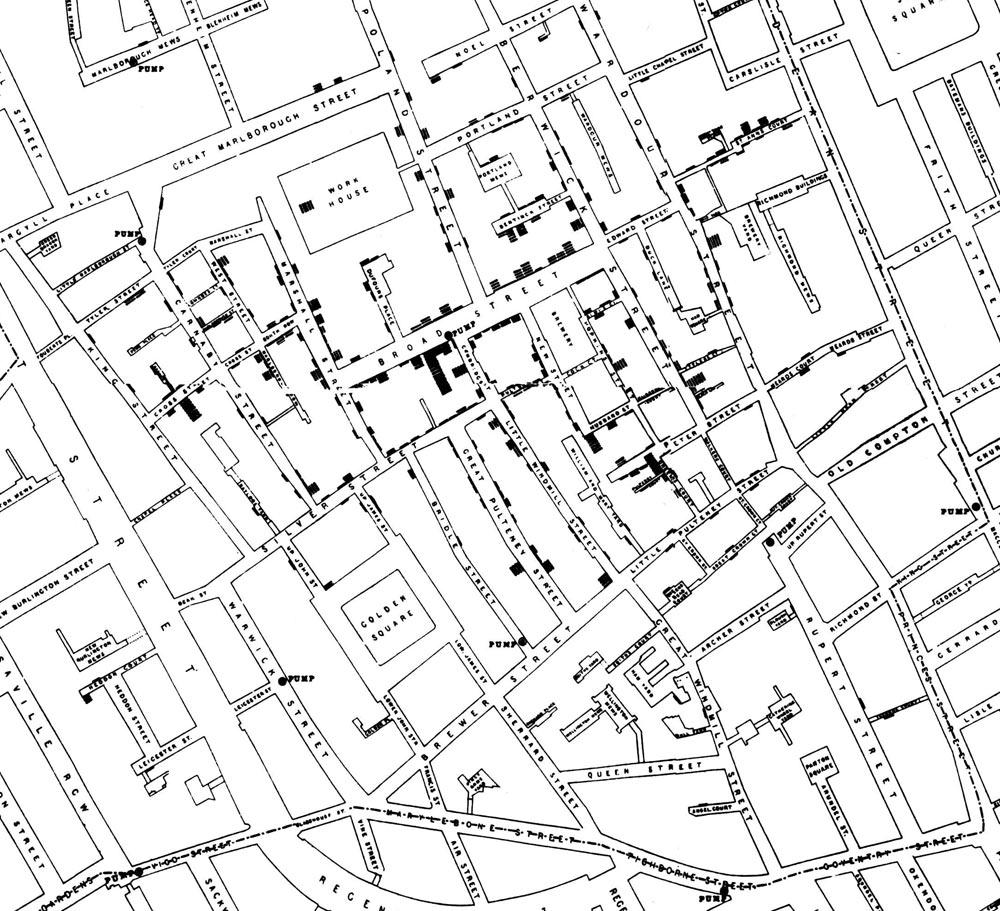
\includegraphics[width=0.5\linewidth]{images/John-Snows-cholera-map-of-009} \end{center}

Welcome to \emph{Concepts \& Applications in Spatial Epidemiology (EPI 563)}! This eBook is one of several sources of information and support for your progress through the semester. For an overview of the course, expectations, learning objectives, assignments, and grading, please review the full course syllabus on Canvas. This eBook serves to provide a \emph{`jumping off point'} for the content to be covered each week. Specifically, the content herein will introduce key themes, new vocabulary, and provide some additional detail that is complementary to the \emph{asynchronous} (pre-recorded) video lectures, and foundational to the \emph{synchronous} (in class) work.

\hypertarget{strategy-for-using-this-ebook}{%
\section*{Strategy for using this eBook}\label{strategy-for-using-this-ebook}}
\addcontentsline{toc}{section}{Strategy for using this eBook}

There is a separate \emph{module} or \emph{chapter} for each week's content. In general, the content within each week's section is divided into two sections focusing on \textbf{spatial thinking} and \textbf{spatial analysis}. This dichotomy does not always hold, but in broad terms you can expect these sections to be more specific to content in class on \emph{Tuesday} versus \emph{Thursday} respectively.

\begin{itemize}
\tightlist
\item
  \emph{Spatial thinking for epidemiology}: This section introduces vocabulary, concepts, and themes that are important to the incorporation of spatialized or geo-referenced data into epidemiologic work. At a minimum, plan to read this content prior to class Tuesday, although you will likely benefit from reading both sections before Tuesday.
\item
  \emph{Spatial analysis for epidemiology}: This section is more focused on data management, visualization, spatial statistics, and interpretation. This content is relevant for our work together on Tuesday's, but is essential for successful work in the Thursday lab activities.
\end{itemize}

Please note that I will be continually updating the eBook throughout the semester, so if you choose to download, please double-check the \textbf{Last updated} date to be sure you have the most recent version.


\includegraphics{images/by-nc-sa.png}\\
This eBook is licensed under the \href{http://creativecommons.org/licenses/by-nc-sa/4.0/}{Creative Commons Attribution-NonCommercial-ShareAlike 4.0 International License}.

\hypertarget{part-getting-ready}{%
\part{Getting ready\ldots{}}\label{part-getting-ready}}

\hypertarget{software-installation}{%
\chapter*{Software installation}\label{software-installation}}
\addcontentsline{toc}{chapter}{Software installation}

The information in this module follow on the pre-class video on setting up \texttt{R} and \texttt{RStudio} on your computer.

\hypertarget{installing-r-on-your-computer}{%
\section*{\texorpdfstring{Installing \texttt{R} on your computer}{Installing R on your computer}}\label{installing-r-on-your-computer}}
\addcontentsline{toc}{section}{Installing \texttt{R} on your computer}

As of August 2020, the most up-to-date version of \texttt{R} is 4.0.2. The \emph{R Project for Statistical Computing} are continually working to update and improve \texttt{R}, and as a result there are new versions 1-2 times per year.

If you already have \texttt{R} installed, you can open the console and check your current version by doing this: \texttt{R.Version()\$version.string}

If you do not have \texttt{R} or have an older version than 4.0 you can install \texttt{R} by going to the \texttt{R} repository: \url{https://www.r-project.org/}. Note that there are many `mirrors' or servers where the software is stored. Generally it is wise to select one that is geographically close to you, although any should work in theory. One mirror that is relatively close to Atlanta is here: \url{http://archive.linux.duke.edu/cran/}

\hypertarget{installing-rstudio-on-your-computer}{%
\section*{Installing RStudio on your computer}\label{installing-rstudio-on-your-computer}}
\addcontentsline{toc}{section}{Installing RStudio on your computer}

The current version of RStudio 1.3.1056. If you do not have RStudio or have a version older than 1.2 please install/update.

\begin{rmdcaution}{caution}
testing a caution note

\end{rmdcaution}

\textbf{TO INSTALL}: go to \url{https://www.rstudio.com/products/rstudio/download/}

\textbf{TO UPDATE}: Open RStudio and go to Help Menu and choose `Check for Updates'

\hypertarget{installing-packages-for-this-course}{%
\chapter*{Installing packages for this course}\label{installing-packages-for-this-course}}
\addcontentsline{toc}{chapter}{Installing packages for this course}

While base \texttt{R} has a great deal of essential functionality, most of the power of \texttt{R} comes from the rapidly growing list of user-created and contributed `packages'. A package is simply a bundle of functions and tools, sometimes also including example datasets, basic documentation, and even tutorial `vignettes'. You can see all the official \texttt{R} packages by going here: \url{https://cran.r-project.org/web/packages/}.

The most common way to install package in \texttt{R} is with the \texttt{install.packages()} command. For instance to install the package \texttt{ggplot2} you do this:

\texttt{install.packages("ggplot2")}

Notice that for \texttt{install.packages()} you need quotes around the package name. Remember that you only need to install a package once (although you may have to update packages occasionally -- see the green Update button in the Packages tab in R Studio). When you want to actually \emph{use} a package (for example \texttt{ggplot2}) you call it like this:

\texttt{library(ggplot2)}

Notice that for the \texttt{library()} function you \textbf{do not} need quotes around the package name (unlike the \texttt{install.packages()} above). If your call to \texttt{library()} is working, nothing visible happens. However if you see errors, they might be because your package is out of date (and thus needs to be updated/reinstalled), or because some important \emph{dependencies} are missing. Dependencies are other packages on which this package depends. Typically these are installed by default, but sometimes something is missing. If so, simply install the missing package and then try calling \texttt{library(ggplot2)} again.

While \textbf{most} packages can be installed as mentioned above (e.g.~using \texttt{install.packages()}), there are instances where an installation requires additional \emph{tools}, for instance to install from source or from github. Luckily there is a package for that! It is called \texttt{Rtools}, and you should install that \textbf{before} you install the packages below.

\begin{rmdcaution}{caution}
As you submit each installation request, note the output. If you get a warning that says installation was not possible because you are missing a package \emph{`namespace'}, that suggests you are missing a dependency. Try installing the pacakge mentioned in the error. If you have trouble, reach out to the TA's!

\end{rmdcaution}

\hypertarget{installing-rtools40}{%
\section*{\texorpdfstring{Installing \texttt{Rtools40}}{Installing Rtools40}}\label{installing-rtools40}}
\addcontentsline{toc}{section}{Installing \texttt{Rtools40}}

If your laptop uses a Windows operating system, you may need \texttt{Rtools40} installed. This is a supplemental package that resides \emph{outside} of \texttt{R} but is needed to install some packages from source code. However it appears that if you have a MacOS, these tools are already built-in. So you \emph{do not need \texttt{Rtools40}} for Mac.

If you are running Windows, navigate to this website: \url{https://cran.r-project.org/bin/windows/Rtools/} and follow the instructions specific to your operating system.

\hypertarget{installing-packages-used-for-general-data-science}{%
\section*{Installing packages used for general data science}\label{installing-packages-used-for-general-data-science}}
\addcontentsline{toc}{section}{Installing packages used for general data science}

For the rest of this page, copy and paste the provided code in order to install packages necessary for this course. Notice if you hover to the right of a code-chunk in the html version of the eBook, you will see a \emph{copy} icon for quick copying and pasting.

These packages will support some of our general work in \texttt{R}, including working with \texttt{RMarkdown} and R Notebooks, as well as data manipulation tools from the \texttt{tidyverse}. You can learn more about the \texttt{tidyverse} here: \url{https://tidyverse.tidyverse.org/}. The \texttt{tidyverse} is actually a collection of data science tools including the visualization/plotting package \texttt{ggplot2} and the data manipulation package \texttt{dplyr}. For that reason, when you \texttt{install.packages(\textquotesingle{}tidyverse\textquotesingle{})} below, you are actually installing \emph{multiple} packages! The packages \texttt{tinytex}, \texttt{rmarkdown}, and \texttt{knitr} are all necessary for creating \texttt{R} Notebooks, which is the format by which many assignments will be submitted.

\begin{Shaded}
\begin{Highlighting}[]
\FunctionTok{install.packages}\NormalTok{(}\StringTok{\textquotesingle{}tidyverse\textquotesingle{}}\NormalTok{)   }
\FunctionTok{install.packages}\NormalTok{(}\FunctionTok{c}\NormalTok{(}\StringTok{\textquotesingle{}tinytex\textquotesingle{}}\NormalTok{, }\StringTok{\textquotesingle{}rmarkdown\textquotesingle{}}\NormalTok{, }\StringTok{\textquotesingle{}knitr\textquotesingle{}}\NormalTok{)) }
\NormalTok{tinytex}\SpecialCharTok{::}\FunctionTok{install\_tinytex}\NormalTok{()  }
\CommentTok{\# this function installs the tinytex LaTex on your}
\CommentTok{\#  computer which is necessary for rendering (creating) PDF\textquotesingle{}s }
\end{Highlighting}
\end{Shaded}

\hypertarget{installing-packages-use-for-geographic-data}{%
\section*{Installing packages use for geographic data}\label{installing-packages-use-for-geographic-data}}
\addcontentsline{toc}{section}{Installing packages use for geographic data}

There are many ways to get the data we want for spatial epidemiology into \texttt{R}. Because we often (but don't always) use census geographies as aggregating units, and census populations as denominators, the following packages will be useful. They are designed to quickly extract both geographic boundary files (e.g.~\emph{`shapefiles'}) as well as attribute data from the US Census website via an API. \textbf{NOTE}: For these to work you have to request a free Census API key. Notice the \texttt{help()} function below to get instructions on how to do this.

\begin{Shaded}
\begin{Highlighting}[]
\FunctionTok{install.packages}\NormalTok{(}\FunctionTok{c}\NormalTok{(}\StringTok{\textquotesingle{}tidycensus\textquotesingle{}}\NormalTok{,}\StringTok{\textquotesingle{}tigris\textquotesingle{}}\NormalTok{)) }

\FunctionTok{help}\NormalTok{(}\StringTok{\textquotesingle{}census\_api\_key\textquotesingle{}}\NormalTok{,}\StringTok{\textquotesingle{}tidycensus\textquotesingle{}}\NormalTok{)}
\end{Highlighting}
\end{Shaded}

\hypertarget{installing-packages-used-for-spatial-data-manipulation-visualization}{%
\section*{Installing packages used for spatial data manipulation \& visualization}\label{installing-packages-used-for-spatial-data-manipulation-visualization}}
\addcontentsline{toc}{section}{Installing packages used for spatial data manipulation \& visualization}

This section installs a set of tools specific to our goals of importing, exporting, manipulating, visualizing, and analyzing spatial data. The first line of packages have functions for defining, importing, exporting, and manipulating spatial data. The second line has some tools we will use for visualizing spatial data (e.g.~making maps!).

\begin{Shaded}
\begin{Highlighting}[]
\FunctionTok{install.packages}\NormalTok{(}\FunctionTok{c}\NormalTok{(}\StringTok{\textquotesingle{}sp\textquotesingle{}}\NormalTok{, }\StringTok{\textquotesingle{}sf\textquotesingle{}}\NormalTok{, }\StringTok{\textquotesingle{}rgdal\textquotesingle{}}\NormalTok{, }\StringTok{\textquotesingle{}rgeos\textquotesingle{}}\NormalTok{, }\StringTok{\textquotesingle{}maptools\textquotesingle{}}\NormalTok{, }\StringTok{\textquotesingle{}OpenStreetMap\textquotesingle{}}\NormalTok{))  }
\FunctionTok{install.packages}\NormalTok{(}\FunctionTok{c}\NormalTok{(}\StringTok{\textquotesingle{}tmap\textquotesingle{}}\NormalTok{, }\StringTok{\textquotesingle{}tmaptools\textquotesingle{}}\NormalTok{, }\StringTok{\textquotesingle{}ggmap\textquotesingle{}}\NormalTok{, }\StringTok{\textquotesingle{}shinyjs\textquotesingle{}}\NormalTok{, }\StringTok{\textquotesingle{}shiny\textquotesingle{}}\NormalTok{, }\StringTok{\textquotesingle{}micromap\textquotesingle{}}\NormalTok{)) }
\end{Highlighting}
\end{Shaded}

\hypertarget{installing-packages-used-for-spatial-analysis}{%
\section*{Installing packages used for spatial analysis}\label{installing-packages-used-for-spatial-analysis}}
\addcontentsline{toc}{section}{Installing packages used for spatial analysis}

Finally these are packages specifically to spatial analysis tasks we'll carry out.

\begin{Shaded}
\begin{Highlighting}[]
\FunctionTok{install.packages}\NormalTok{(}\FunctionTok{c}\NormalTok{(}\StringTok{\textquotesingle{}spdep\textquotesingle{}}\NormalTok{, }\StringTok{\textquotesingle{}CARBayes\textquotesingle{}}\NormalTok{, }\StringTok{\textquotesingle{}sparr\textquotesingle{}}\NormalTok{, }\StringTok{\textquotesingle{}spatialreg\textquotesingle{}}\NormalTok{,  }\StringTok{\textquotesingle{}DCluster\textquotesingle{}}\NormalTok{))}
\FunctionTok{install.packages}\NormalTok{(}\FunctionTok{c}\NormalTok{(}\StringTok{\textquotesingle{}GWmodel\textquotesingle{}}\NormalTok{, }\StringTok{\textquotesingle{}spgwr\textquotesingle{}}\NormalTok{) )}
\end{Highlighting}
\end{Shaded}


  \bibliography{book.bib}

\end{document}
